% !TeX encoding = UTF-8
% !TeX root = V29_AFM.tex
% !TeX spellcheck = de_DE_frami

\section{Einleitung}
Die Rasterkraftmikroskopie (engl. Atomic Force Microscopy, AFM) ist eine Methode, das Profil einer Probe in einem kleinen Bereich zu vermessen, der je nach Gerät von einem $\milli\metre^2$ bis hinab zum Maßstab einzelner Moleküle und Atome reicht. Hierbei tastet eine Spitze an einem Cantilever die Probe ab und ermittelt die Kraft, die diese auf die Spitze ausübt.

Im folgenden werden einige der wichtigsten Messmodi am AFM erklärt, die neben dem Profil teils auch weitere Eigenschaften des Materials an der Oberfläche ergeben; so z.B. den E-Modul und die Adhäsion.

Weiterhin erstellen wir Aufnahmen verschiedener Proben, um Aussagen über deren Struktur sowie Probleme der AFM treffen zu können. 

\newpage
\section{Theorie}
\subsection{Wechselwirkungspotentiale}
Die zeitlichen Fluktuationen in der Elektronenwolke eines Atoms sind zufällig, wodurch der negative Ladungsschwerpunkt des Atoms mit dem positiv geladenen Atomkern zusammenfällt. Folglich kann das fluktuierende elektrische Feld an sich keine Kraft auf andere Ladungen ausüben. Betrachtet man allerdings mehrere Atome, so induziert das kurzlebige Dipolmoment $\vec p$ in den anderen Atomen ein gleichgerichtetes Dipolmoment $\vec p_i \sim \vec p$. Es bildet sich zu jedem Zeitpunkt eine  vorherrschende Orientierung der $\vec p_i$ heraus, was eine anziehende Kraft bedingt, die Van-der-Waals-Kraft, welche mit dem Atomabstand$r$ gemäß $r^{-7}$ abfällt. Daraus ergibt sich ein Potential der Form $r^{-6}$.

Bei zu starker Annäherung der Atome überwiegen abstoßende Kräfte, die aus der Coulomb-Kraft $F_C$ und der Pauli-Abstoßung zwischen den sich durchdringenden Elektronenwolken folgen. Das zugehörige Potential fallen in etwa mit $r^{-12}$ ab.

Die Wechselwirkungs lässt sich folglich typischerweise relativ gut durch das Lennard-Jones 6-12-Potential beschreiben, hierbei ist $c$ eine Konstante und $r_0$ der Gleichgewichtsabstand der Atome:
\begin{equation}
  V_{LJ} = c \cdot \left[ \left(\tfrac{r_0}{r}\right)^{12} - 2 \cdt \left(\tfrac{r_0}{r}\right)^{6} \right]
\end{equation}

Im Falle der AFM betrachten wir die Wechselwirkung zwischen einer näherungsweise ebenen Probe und einer als Halbkugel\footnote{Für hochauflösende Messungen kann es sich um eine einzelnes Atom an der Spitze handeln.} angenommenen Spitze. Für diese Anordnung ergibt sich für das Van-der-Waals-Potential eine Abhängigkeit von $1/h$ \cite[S. 5]{lit:hampp}, wobei $h$ die Höhe der Spitze über der Probe bezeichnet. Insgesamt erhalten wir folglich mit zwei Konstanten $A, B$ ein Potential
\begin{equation}
  V =  - A \cdt h^{-1} + B \cdt h^{-12} \label{eq:V_Spitze}
\end{equation}

Die Kraft $F = - \ddp{V}{h}$ auf die Spitze führt zum Biegen des Cantilevers, der als Blattfeder mit Federkonstante $k$ beschrieben werden kann. Die senkrechte Durchbiegung $s$ ergibt sich aus dem Hooke'schen Gesetz
\begin{equation}
  F =  k \cdot s	\iff	s = F \div k
\end{equation}
Dabei ist anzumerken, dass die Höhe $h$ der Spitze über der Probe sich aus der Position $z$ des Cantilevers und dessen Durchbiegung $s$ zusammensetzt:
\begin{equation}
  h = z - s
\end{equation}


\subsection{Kraft-Distanz-Kurve}
Die schematische Kraft-Distanz-Kurve in Abbildung \ref{fig:Fz} zeigt die auf die Spitze wirkende Kraft in Funktion von $z$. Links ist die Anziehung vernachlässigbar. Der Sprung in der Mitte wird als Snap In bezeichnet, bei dem die anziehende Kraft den Cantilever so lange verbiegt, bis die Spitze in Kontakt ist ($h = h_0$). Anschließend wird die Spitze immer stärker gegen die Probe gedrückt, der dargestellte lineare Anstieg gilt näherungsweise, solange sowohl Cantilever als auch Probe nur elastisch verformt werden.

Beim Zurückziehen der Spitze haftet diese bereits an der Probe, weshalb eine stärkere Gegenkraft der Blattfeder erforderlich ist als zuvor: Das Zurückspringen erfolgt bei einem etwas größeren Abstand als der Snap In.

\begin{figure}[h]
	\centering
	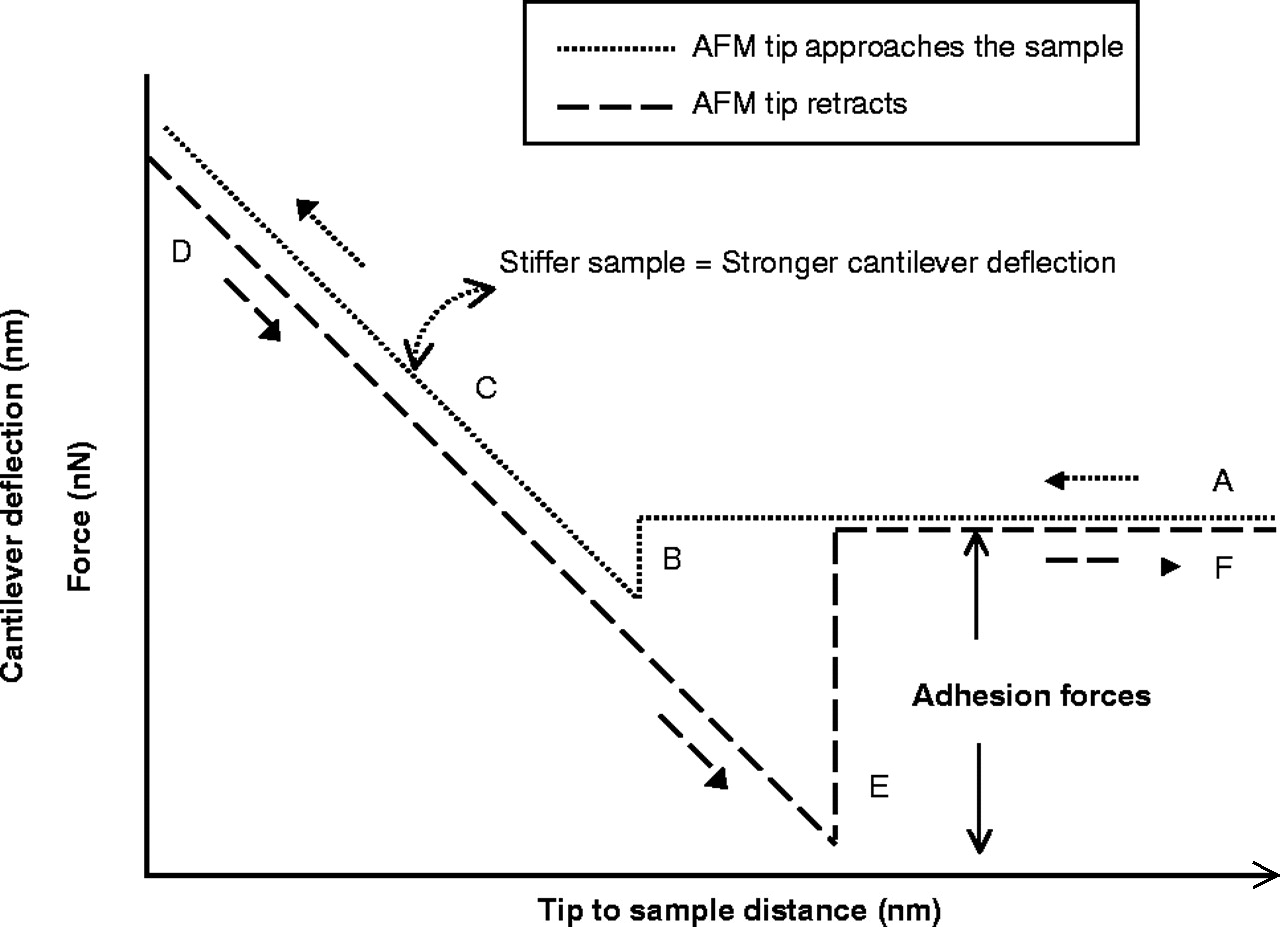
\includegraphics[width=0.8\textwidth]{Fz.png}
	\caption{Kraft-Distanz-Kurve für Annäherung und Entfernung von der Probe \cite{lit:Fz}}
	\label{fig:Fz}
\end{figure}

Ist die Oberfläche mit Wasser benetzt, so führt die Kapilliarkraft zu einem nochmals deutlich stärkeren Adhäsion und folglich einem größeren Unterschied zwischen Annäherung und Zurückziehen.

\subsection{Mess-Modi}
\subsubsection{Contact mode}
Die einfachste Möglichkeit zur Messung ist der contact mode, bei dem die Spitze anschaulich betrachtet die Probe berührt. Von Vorteil ist insbesondere, dass unterhalb des Gleichgewichtsabstands $h_0$ starke abstoßende Kräfte wirken und der Snap In bereits erfolgt ist. 

Dabei wird üblicherweise eine der folgenden zwei Konfigurationen verwendet (Bei Proben mit extremer Topologie wird bei constant height das Abbrechen der Spitze riskiert):
\begin{description}
 \item[constant height:] Die Position $z$ des Cantilevers bleibt konstant, das Messsignal entspricht der gemessenen Kraft.
 \item[constant force:] Die Position $z$ des Cantilevers wird nachgesteuert, um die Kraft auf einem vorgegebenen Wert zu halten.
\end{description}

Da die Spitze gegen die Probe gedrückt wird, ist dieses Verfahren nicht für weiche Materialien (z.B. zahlreche organische Proben) nutzbar.

\subsubsection{Noncontact mode}
Für $h > h_0$, den sogenannten non contact mode, wird die Spitze zur Probe gezogen. Allerdings gibt es durch den Snap In keinen Bereich, in dem diese anziehenden Kräfte statisch gemessen werden können -- der Cantilever biegt sich zur Probe hin und berührt diese. Aus diesem Grund wird die Spitze mittels eines Piezoelements einer hochfrequenten Schwingung unterworfen, wodurch die Spitze vor dem Snap In bereits zurückschnellt.

Während dieses Verfahren auch für empfindliche Materialien gut geeignet ist, täuscht eine Flüssigkeitsschicht auf der Probe (Für Abbildung \ref{fig:Si_force-distance} entsteht dieser durch das Anhauchen.) vor, Teil der Probe zu sein und wird folglich   mit erfasst.

\subsubsection{Tapping mode}
 Eine dritte Anordnung ist der tapping bzw. intermittent mode, bei dem der Cantilever ebenfalls oszilliert, allerdings aber bei jeder Schwingung die Probe berührt. Dabei lässt sich aus der Modulation der Schwingungsfrequenz die durch die Probe bedingte Dämpfung und somit deren lokales E-Modul ermitteln.


In Abbildung \ref{fig:Potential} sind das auf die Spitze wirkenden Potential aus Gleichung \eqref{eq:V_Spitze} sowie die für verschiedene Messmodi genutzten Bereiche des Potentials dargestellt.


\begin{figure}[p]
	\centering
	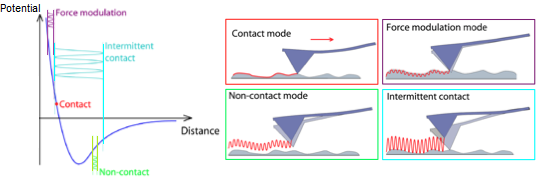
\includegraphics[width=\textwidth]{AFM-fig3.png}
	\caption[Potential $V(h)$ einer Ebene auf die Spitze]
		     {Potential $V(h)$ einer Ebene auf die Spitze. \cite{lit:grenoble} bzw. \cite{lit:jpk}\\
			Einordnung der Messmodi (contact, noncontact, tapping) in den Graphen.}
	\label{fig:Potential}
\end{figure}

\subsection{Steuerung}
Die Position $(x,y,z)$ des Cantilevers über der Probe lässt sich bei Rasterkraft-Mikroskopen mittels Piezo-Elementen einstellen. Dabei handelt es sich um Kristalle ohne Inversionssymmetrie, bei denen der positive und negative Ladungsschwerpunkt der Elementarzelle mittels einer äußeren Spannung getrennt werden können, was zu einer Verformung der Zelle und somit des Kristalls führt. Da eine winzige Ladungstrennung bereits ein relativ starkes $E$-Feld aufbaut, lässt sich die Längenänderung mit der geforderten Präzision (\pico\metre{} bis \micro\metre) durch Anlegen entsprechend geringer Spannungen erzielen. Dabei reagieren Piezo-Elemente im Bereich bis 1V nahezu linear, die Abweichung ist gegenüber den anderen Artefakten vernachlässigbar.

Neben der ursprünglich verwendeten Dreibein-Anordnung, in der je ein Piezo eine Koordinate ansteuert, werden inzwischen  zahlreiche Geräte (einschließlich des hier verwendeten easyScan E-AFM) mit Piezo-Rohrscannern ausgestattet. In Abbildung \ref{fig:tube} ist die Ansteuerung eines solchen Scanners dargestellt:\\
Die zentrale $z$-Elektrode steuert die axiale Elongation/Kontraktion, über die vier äußeren Elektroden kann eine Biegung in $x$- bzw. $y$-Richtung erzielt werden. 

Das Oberflächenprofil wird linienweise entlang der $x$-Achse abgetastet; dabei ist die Scan-Richtung typischerweise abwechselnd vorwärts und rückwärts, wodurch der Cantilever eine schleifenförmige Bahn abfährt. Nur wenn immer in der gleichen Richtung über eine Kante gescannt werden soll, wird dies auf eine der Scan-Richtungen beschränkt.


\begin{figure}[p]
	\centering
	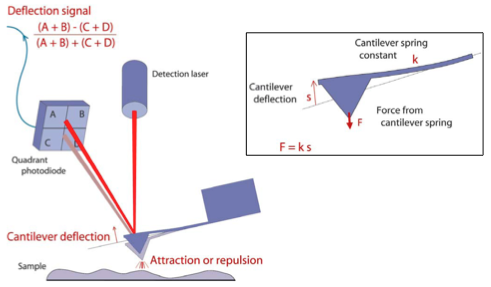
\includegraphics[width=0.8\textwidth]{AFM-fig1.png}
	\caption{Optische Bestimmung der auf den Cantilever wirkenden Kraft $F$. \cite{lit:grenoble}.}
	\label{fig:laser}
\end{figure}

\begin{figure}[p]
	\centering
	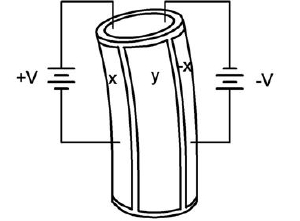
\includegraphics[width=0.5\textwidth]{piezo_tube.jpg}
	\caption{Piezo-Rohrscanner zur Positionierung der Spitze \cite{lit:tube}}
	\label{fig:tube}
\end{figure}

Wie in Abbildung \ref{fig:laser} ersichtlich, wird die Auslenkung $s$ des Cantilevers über einen schräg einfallenden und am Cantilever reflektierten Laser kontrolliert. Der reflektierte Laserstrahl trifft auf eine viergeteilte Diode, die aus der Verschiebung der Intensität zwischen den vier Sektoren die Kraft $F \sim s$ berechnet.

Da in diesem Versuch mit contact mode, constant force durchgeführt wird, ist eine Rückkopplung des Kraft-Signals zum $z$-Piezo notwendig. Hierfür definieren wir
\begin{description}
\item[P-Gain:] Um dem Höhenprofil ohne Kollision folgen zu können, wird eine direkte Rückkopplung benötigt, die z.B. bei einer steigenden Flanke sofort $z$ proportional zu $F$ erhöht. Die Stärke dieses \emph{proportionellen} Feedbacks wird mit dem Koeffizienten P-Gain gewichtet.
\item[I-Gain:] Zusätzlich zur Reaktion auf Höhenänderungen muss der Piezo weiterhin die bisherige $z$-Position erhalten; ohne diese Komponente würde der Piezo immer wieder in die Ruhelage zurückgehen. Da sich die aktuelle Position aus der Summe aller bisherigen Reaktionen $\int\! F \,\d t$ ergibt, bezeichnet man den Koeffizienten für dieses \emph{integrale} Feedback als I-Gain.
\end{description}

\begin{figure}[p]
	\centering
	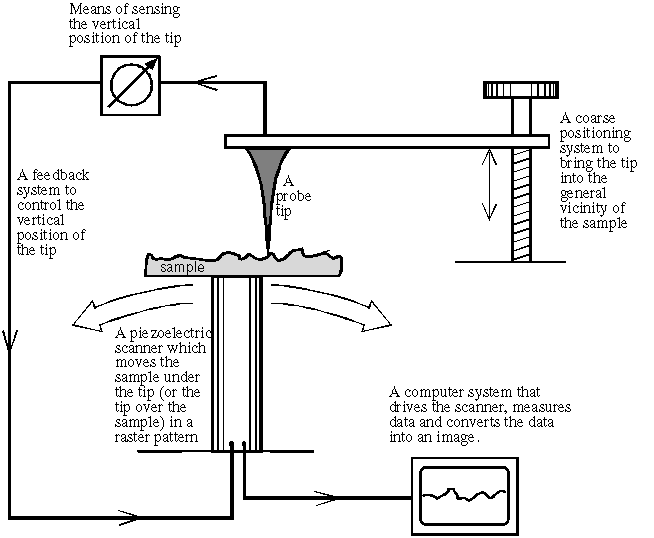
\includegraphics[width=\textwidth]{regelkreis.png}
	\caption{Schematischer Aufbau des Regelkreises eines Rasterkraftmikroskops \cite{lit:guide}.}
			Nach der groben Einstellung der Höhe wird diese während der Messung durch das Feedback des Kraftsensors automatisch nachreguliert.
	\label{fig:feedback}
\end{figure}

\subsection{Artefakte}
% Piezo: sin x != x
% Piezo: minimal nichtlinear
% Piezo: Hysterese
% Spitze: doppelt, dreckig, gebrochen
% Cantilever; gealtert, Feinriß
% thermischer Drift, Gebäudeschwingungen
% speed: edge overshoot